\documentclass[a4paper,11pt]{article}
\usepackage[utf8]{inputenc}
\usepackage[paper=a4paper, hmargin=1.5cm, bottom=1.5cm, top=3.5cm]{geometry}
\usepackage[T1]{fontenc}
\usepackage[colorlinks=true, linkcolor=blue]{hyperref} %Links para el indice.
\usepackage{amsfonts}
\usepackage{verbatim}
\usepackage{listings}
\usepackage{caption}
\usepackage{subcaption}
\usepackage{graphicx}
\usepackage{wrapfig}
\usepackage[section]{placeins}
\usepackage{float}
%\usepackage{adjustbox}
\usepackage{amsmath}
\usepackage{blindtext}
\usepackage{sidecap}
\usepackage{color}

\captionsetup[subfigure]{labelformat=empty}

% \newcommand{\real}{\hbox{\bf R}}

\title{Traceroute}

\begin{document}

\maketitle

\begin{center}
	Universidad de Buenos Aires - Departamento de Computaci\'on - FCEN
\end{center}

\vspace{2cm}
Integrantes:

\begin{itemize}
	\item Gallardo, Guillermo L.U.: 32/10 \verb+gagdiez.c@gmail.com+
	\item Fixman, Martin L.U.: 391/11 \verb+martinfixman@gmail.com+
	\item Matayoshi, Leandro L.U.: 79/11 \verb+leandro.matayoshi@gmail.com+
	\item Szyrej, Alexander L.U.: 642/11 \verb+alexander.szyrej@gmail.com+
		
\end{itemize}

\newpage

\tableofcontents

\newpage

\section{Introducción}

\subsection{Objetivos generales}

ICMP es el m\'odulo del protocolo TCP/IP que se encarga de proveer mensajes de error y de control cuando
se produce alguna anormalidad en el env\'io de un datagrama IP. Existen distintas herramientas
que se apoyan sobre este m\'odulo para obtener informaci\'on acerca del estado de las rutas que
debe atravesar un paquete para llegar al destino, como por ejemplo, el valor del RTT (round-trip-time)
entre 2 hosts. Entre estas herramientas se destacan los comandos \emph{ping} y \emph{traceroute}.

El objetivo de este trab\'ajo pr\'actico es realizar nuestra propia
implementaci\'on de \emph{traceroute} y utilizar la misma para comprender el
funcionamiento de las comunicaciones a larga distancia sobre internet.
Para esto \'ultimo realizaremos un an\'alisis de la distribuci\'on
geogr\'afica del conjunto de enlaces y routers atravesados por los paquetes
ICMP.
A su vez intentaremos detectar cuando dichos paquetes atraviesan enlaces
intercontinentals utilizando solamente los valores de los RTT.

Por todos estos motivos, los hosts destino de los paquetes son cuatro universidades ubicadas en
otros continentes, las mismas son:

\begin{quote}
\begin{description}
	\item [$\bullet$ Oxford] {University of Oxford, Londres, Reino Unido}
	\item [$\bullet$ MSU] {\foreignlanguage{russian}{Московский государственный университет} (Universidad Estatal de Mosc\'u), Mosc\'u, Federaci\'on Rusa}
	\item [$\bullet$ Queensland] {University of Queensland, Queensland, Australia}
	\item [$\bullet$ Tsinghua] {\begin{CJK}{UTF8}{gbsn}清华大学\end{CJK} (Universidad de Tsinghua), Beijing, Rep\'ublica Popular China}
\end{description}
\end{quote}

\subsection{Tipos de mensajes ICMP}

Los mensajes de ICMP se transmiten en forma de datagramas. El emisor puede ser tanto un host como router,
y el destino es siempre la direcci\'on source del datagrama IP que motiv\'o el mensaje.

Entre los tipos de mensajes de error m\'as comunes se destacan:
\begin{itemize}
  \item Echo reply: Respuesta a echo request. Los datos recibidos por el request deben ser inclu\'idos
  en el mensaje. type: 0
  \item Destination host unreachable: El router no encuentra en su tabla una direcci\'on a la cual
  forwardear el paquete. type: 3
  \item Redirect: El router que recibe el paquete detecta que otro router ofrece un camino m\'as
  efectivo para forwardear el paquete. type: 5
  \item Echo request: Se espera que los datos enviados sean recibidos nuevamente en un mensaje echo
  reply. type: 8
  \item Time exceeded: Mensaje generado por un router para indicarle al host emisor de un datagrama
  que su TTL (''Time to live'') ha alcanzado el valor 0.

\end{itemize}


\subsection{Ping}

El comando ping es una tool que permite testear la actividad de un host dentro del protocolo IP y medir
el RTT entre el dispositivo que ha ejecutado el comando y el host de inter\'es. El mismo se basa en
la emisi\'on de mensajes \emph{echo request}, y sus respectivas respuestas \emph{echo reply}. El RTT queda
determinado entonces por el tiempo que tarda el host emisor en recibir la respuesta.
Los requests para los cuales no se recibe ninguna respuesta son registrados como paquetes perdidos.

\subsection{Traceroute}

A diferencia de ping, \emph{traceroute} provee informaci\'on acerca de la ruta que siguen los datagramas
para arribar al destino. Esta herramienta arma un registro ordenado con los routers que ha atravesado
el paquete, junto con el valor de los RTT para cada uno de ellos.
En la siguiente secci\'on explicaremos el
mecanismo de esta herramienta con mayor detalle.


\section{Desarrollo}

%Más especificamente, \textcolor{red}{estimamos un RTT medio} para cada salto que
se da en la ruta que nos comunica con cada host, y \textcolor{red}{normalizamos
este valor para conseguir el Z-score de los RTT (ZRTT)} para cada salto que nos
de suficiente informaci\'on como para \textcolor{red}{analizar el trasfondo del
tr\'afico en la red}.

\begin{figure}[!h]
  \begin{center}
      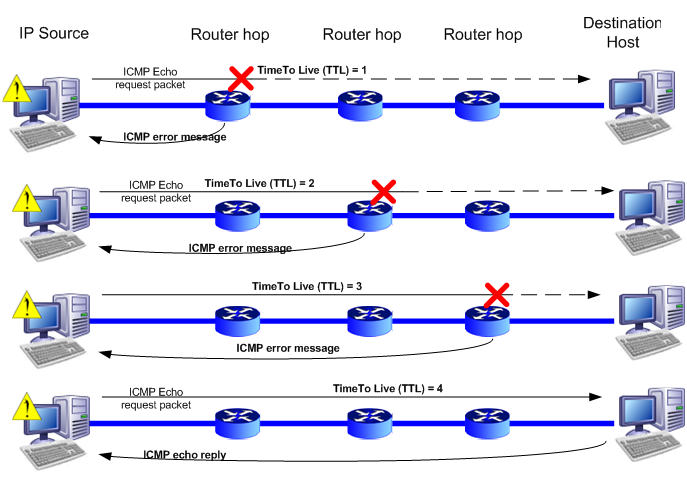
\includegraphics[scale=0.4]{imagenes/traceroute.png}
      \caption{Mecanismo de acción de traceroute}
      \label{fig:contra1}
  \end{center}
\end{figure}

Para analizar las rutas que pueden pasar por cables submarinos, hicimos este
an\'alisis a cuatro universidades:

\begin{itemize}
	\item [MSU] {\foreignlanguage{russian}{Московский государственный
	университет имени М. В. Ломоносова}
	(Universidad Estatal de Mosc\'u) Federaci\'on Rusa}
	\item [Oxford] {University of Oxford, Reino Unido}
	\item [Queensland] {University of Queensland, Australia}
	\item [Tsinghua] {\foreignlanguage{chinese}{清华大学} (Universidad de Tsinghua), China}
\end{itemize}

Por cada host, se env\'ian 10 paquetes con \textit{Time to Live} diferente hasta
llegar al host indicado, y se toma la media estad\'istica de el \textit{Round
Trip Time} de cada tramo.

Hay muchos hosts donde la acci\'on de responder paquetes ICMP se le da
much\'isima menor prioridad que la acci\'on de forwardearlos a otro host. Por
esta raz\'on hay muchos hosts que dan un \textit{Round Trip Time} mayor a otro
host a pesar de ser m\'as ``cercanos'' en la red y fisicamente al cliente.
Aunque en la mayor\'ia de los hosts esto no cambia mucho nuestros resultados (ya que
solo queremos buscar links continentales), hay algunos hosts donde la diferencia
entre RTT dado y el real es demasiado alta. Por esta raz\'on solo tomamos
paquetes con un RTT menor a \textbf{1 segundo}, e ignoramos los hosts donde
todos los 10 paquetes fueron ignorados.


\clearpage

\section{Resultados y análisis}

%\input{resultado.tex}

\section{Conclusiones}

%Como resultado de la información presentada, concluimos que el valor de ZRTT de un enlace es útil para dar una idea de la distancia que este recorre. 

Tomamos algunos valores como limite para valores significativos de ZScore (el umbral) y nos quedamos con aquel que consideramos mas pertinente en todos los casos. Este umbral ser\'a tal que los enlaces para todos los tracerouteos que tienen un score por arriba de ese umbral tienen buenas chances de ser enlaces submarinos, es decir, recorrer distancias bastante extensas.

Aun as\'i encontramos enlaces que incluso teniendo un ZRTT que supera el umbral, no se caracterizan por ser enlaces submarinos, por lo que concuimos que el ZRTT no sirve para caracterizar al cien por ciento dichos enlaces.



\section{Referencias}
\begin{itemize}
%	\item \textbf{Computer Networks: A Systems Approach}, \textit{Larry L. Peterson and Bruce S. Davie.}
%	\item \textbf{Computer Networks}, \textit{Andrew S. Tanenbaum}
%	\item \textbf{Special-Purpose IP Address Registries} (RFC 6890), \textit{Internet Engineering Task Force (IETF)}
%	\item \textbf{An Ethernet Address Resolution Protocol or Converting Network Protocol Addresses to 48.bit Ethernet Address for Transmission on Ethernet Hardware} (RFC 826), \textit{David C. Plummer}
\end{itemize}

\end{document}
